% /*@@
%   @file      rotating_sym.tex
%   @date      6 June 2002
%   @author    Denis Pollney
%   @desc 
%              Description of the implementation of `rotating'
%              symmetry conditions in CartGrid3D.
%   @enddesc 
%   @version $Header$
% @@*/

\documentclass{article}

\newif\ifpdf
\ifx\pdfoutput\undefined
\pdffalse % we are not running PDFLaTeX
\else
\pdfoutput=1 % we are running PDFLaTeX
\pdftrue
\fi

\ifpdf
\usepackage[pdftex]{graphicx}
\else
\usepackage{graphicx}
\fi

\parskip = 0 pt
\parindent = 0pt
\oddsidemargin = 0 cm
\textwidth = 16 cm
\topmargin = -1 cm
\textheight = 24 cm

\begin{document}

\title{Rotating symmetry conditions}
\author{Denis Pollney}
\date{June 2002}

\maketitle

\begin{abstract}
These notes describe the implentation of rotating symmetry conditions
for \emph{bitant} and \emph{quadrant} domains in \texttt{CartGrid3D}.
For these particular domain types, the condition that fields on the
grid have a rotational symmetry in a plane along one of the
coordinate axes can be simply implemented with minor extensions to the
already existing symmetry mechanism, which copies the components of
a given field to the required ghost-zones with a possible plus-minus
inversion.
\end{abstract}

%------------------------------------------------------------------------------
\section{Introduction}
\label{sec:rs_intro}
%------------------------------------------------------------------------------

A number of useful physical models involve situations where a
rotational symmetry is present in all of the relevant fields. By
`rotational symmetry' we mean that there exists a pair of half-planes
extending from one of the coordinate axes and separated by an angle
$\theta$ which have the property that on $A$ and near to $A$ can be
mapped onto $B$ and corresponding points near to $B$ (see Figure
\ref{fig:rs_rotation_examples}).
%
\begin{figure}
\centering
\begin{tabular}{ccc}
\ifpdf
\else
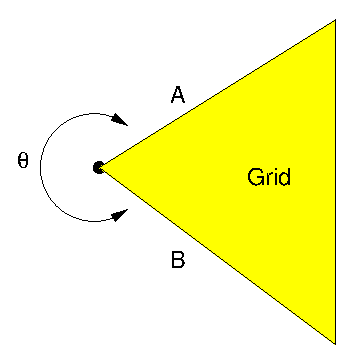
\includegraphics[height=40mm]{fig/rotate_general.eps}
\fi
&
\ifpdf
\else
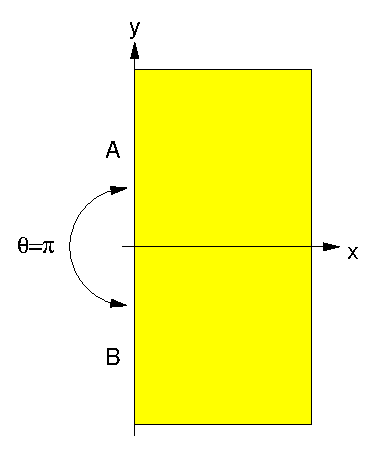
\includegraphics[height=40mm]{fig/rotate_bitant.eps}
\fi
&
\ifpdf
\else
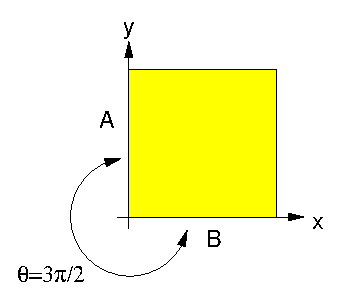
\includegraphics[height=25mm]{fig/rotate_octant.eps}
\fi
\\
(a) & (b) & (c)
\end{tabular}
\caption{Rotational symmetries, looking down the $z$-axis. In the
general case (a), the half-planes $A$ and $B$ are separated by an
angle $\theta$. Data at $A$ can be mapped on to points of $B$ via a
rotation through $\theta$. Particular cases of importance are the
rotation through $\theta=\pi$, so that data on the positive $y$-axis
is mapped onto the negative $y$, and vice versa; and the rotation
through $\theta=3\pi/2$ so that data need be specified only in a
single quarter-plane.}
\label{fig:rs_rotation_examples}
\end{figure}
%
In particular, situations for which such conditions can be useful
include
\begin{itemize}
  \item rotating axisymmetric bodies -- satisfies the rotational 
    symmetry for arbitrary $\theta$.
  \item pairs of massive bodies separated by distances $\pm
    \mathbf{d}$ from the origin and with identical oppositely directed
    momenta $\pm \mathbf{p}$ (Figure \ref{fig:rs_bbh}) -- satisfies
    the half-plane rotational symmetry ($\theta=\pi$) or, if
    $\mathbf{p}=0$ then also the quarter plane symmetry
    ($\theta=3\pi/2$).
\end{itemize}
\begin{figure}
\centering
\ifpdf
\else
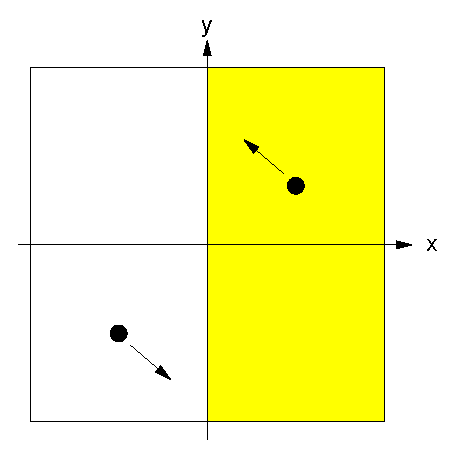
\includegraphics[height=40mm]{fig/rotate_bbh.eps}
\fi
\caption{A physical system consisting of a pair of identical bodies
  separated equal distance along a line through the origin, and moving
  with equal but opposite momenta, can be modelled using only the
  positive half-plane if the rotating symmetry condition is applied to
  the $x=0$ plane.}
\label{fig:rs_bbh}
\end{figure}

In order to apply the boundary condition exactly on a numerical grid,
it is necessary that grid points to each side of the mapping planes
$A$ and $B$ can be mapped onto each other exactly. In particular, this
means that the rotating symmetry conditions can be applied exactly if
the half-planes are each aligned with one of the coordinate axes. For
general planes $A$ and $B$, however, interpolation would be required
to put data in the neighbourhood of $A$ onto grid points near
$B$. Only the particular cases described by Figures
\ref{fig:rs_rotation_examples} (b) and (c) will be
considered here.

%------------------------------------------------------------------------------
\section{Symmetry conditions}
\label{sec:rs_application}
%------------------------------------------------------------------------------

For a given field, the boundary condition is applied as follows. For
each ghost-zone point along the symmetry plane, the corresponding
point on the physical grid (under the rotational $\theta$) is
determined. To determine the value of the ghost-zone point, the
value on the physical grid is simply transformed under the given
rotation.\\

The first of these issues is not difficult to resolve. As an example,
consider the half-plane rotational symmetry about the $z$-axis applied
in the $x=0$ plane, as depicted in Figure \ref{fig:rs_grid}. The
Figure has
$j=0\ldots m$ in the $y$ direction, an arbitrary number of points in the
$x$ and $z$ directions, and some ghostzones whose $j$ coordinates are
labelled $j=-1,-2,\ldots$. Then for the ghost-zone point $(n-i, -j,
k)$, the corresponding physical point under rotation is (1) $(i,j-1,k)$
if the $x=0$ plane is on the grid, or (2) $(i,j,k)$ if the $x=0$ plane
is staggered between a grid point and the first ghost-zone
point. There is an implicit assumption here that the grid extends
exactly the same distance to each side of the rotation axis. \\

\begin{figure}
\centering
\ifpdf
\else
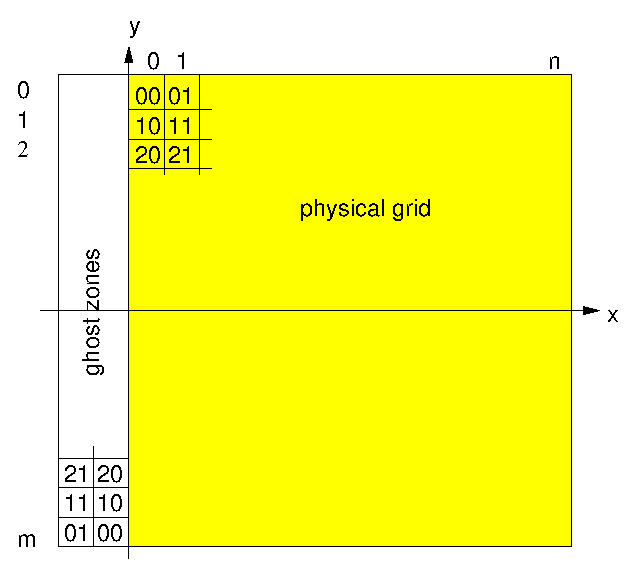
\includegraphics[height=40mm]{fig/rotate_grid.eps}
\fi
\caption{The mapping of physical points onto ghost-zone points for a
  half-plane rotation about the $z$-axis, where the $x=0$ plane is
  staggered between gridpoints, and two ghost zones have been
  allocated.}
\label{fig:rs_grid}
\end{figure}

The remaining issue is to determine how the fields at a point
$(i,j,k)$ are modified under a rotation of a given angle. A set of
basis vectors $(\mathbf{\hat{x}},\mathbf{\hat{y}},\mathbf{\hat{z}})$
can be rotated to an arbitrary direction by applying the rotation
matrix
\begin{equation}
  \mathbf{P} = 
  \left[
    \begin{array}{ccc}
      \eta_1(\cos\theta_1\cos\theta_3 - \sin\theta_1\cos\theta_2\sin\theta_3) &
      \sin\theta_1\cos\theta_3 + \cos\theta_1\cos\theta_2\sin\theta_3 &
      \sin\theta_2\sin\theta_3 \\
      -(\cos\theta_1\sin\theta_3 + \sin\theta_1\cos\theta_2\cos\theta3) &
      \eta_2(\sin\theta_1\sin\theta_3 + \cos\theta_1\cos\theta_2\cos\theta_3) &
      \sin\theta_2\cos\theta_3 \\
      \sin\theta_1\sin\theta_2 &
      -\cos\theta_1\sin\theta_2 &
      \eta_3\cos\theta_2
    \end{array}
  \right],
\end{equation}
which preserves the orthogonality of the basis. The matrix
$\mathbf{P}$ has been written in terms of the Euler angles
$0\leq\theta_1<2\pi$, $0\leq\theta_2<2\pi$, and $0\leq\theta_3<\pi$,
and the factors $\eta_1=\pm 1$, $\eta_2=\pm 1$, $\eta_3=\pm 1$ are
introduced to allow for reflections of individual axes (ie. changes of
handedness of the basis).
The basis is transformed under $\mathbf{P}$ via the matrix multiplication
\begin{equation}
  \left[
    \begin{array}{c}
      \mathbf{\hat{x}^\prime} \\
      \mathbf{\hat{y}^\prime} \\
      \mathbf{\hat{z}^\prime}
    \end{array}
  \right]
  =
  \mathbf{P} 
  \left[
    \begin{array}{c}
      \mathbf{\hat{x}} \\
      \mathbf{\hat{y}} \\
      \mathbf{\hat{z}} 
    \end{array}
  \right].
\end{equation}

Vectors and tensor components are transformed under the given rotation
by applying the $\mathbf{P}$ matrix:
\begin{eqnarray}
  \mathbf{v} & \rightarrow & \mathbf{P}^T \mathbf{v}, \\
  \mathbf{G} & \rightarrow & \mathbf{P}^T \mathbf{G} \mathbf{P},
\end{eqnarray}
where $\mathbf{v}$ is a 3-vector,
\begin{equation}
  \mathbf{v} = [v_x, v_y, v_z]^T,
\end{equation}
and $\mathbf{G}$ is a two-index tensor treated as a matrix,
\begin{equation}
  \mathbf{G} =
    \left[
      \begin{array}{ccc}
	g_{xx} & g_{xy} & g_{xz} \\
	g_{yx} & g_{yy} & g_{yz} \\
	g_{zx} & g_{zy} & g_{zz}
      \end{array}
    \right].
\end{equation}

\emph{Example 1.} The special case of a reflection in the $x=0$ plane
corresponds to an inversion of the $x$-axis, so that
$\theta_1=\theta_2=\theta_3=0$ and $\eta_1=-1$,
\begin{equation}
  \mathbf{P}_{x-\mathrm{reflect}} = \left[
    \begin{array}{ccc}
      -1 & 0 & 0 \\
       0 & 1 & 0 \\
       0 & 0 & 1
    \end{array}
    \right].
\end{equation}

\emph{Example 2.} For a rotation about the $z$ axis by an angle of
$\theta=\pi$ (corresponding to Figure \ref{fig:rs_grid}), the only
non-zero rotation angle is $\theta_1=\pi$, so that
\begin{equation}
  \mathbf{P}_{z-\mathrm{rotate}} = \left[
    \begin{array}{ccc}
      -1 &  0 & 0 \\
       0 & -1 & 0 \\
       0 &  0 & 1
    \end{array}
    \right].
\end{equation}

\emph{Example 3.} A quarter-plane grid with positive $y$-axis values
mapped onto the positive $x$-axis (as in Figure\nobreak~
\ref{fig:rs_rotation_examples}) corresponds non-zero angle
$\theta_1=3\pi/2$, with the resulting rotation matrix
\begin{equation}
  \mathbf{P}_{z-\mathrm{rotate(3/2)}} = \left[
    \begin{array}{ccc}
       0 & -1 & 0 \\
       1 &  0 & 0 \\
       0 &  0 & 1
    \end{array}
    \right].
\end{equation}

%------------------------------------------------------------------------------
\section{Implementation}
\label{sec:rs_implementation}
%------------------------------------------------------------------------------

In order to implement the bitant, quadrant and octant
\emph{reflection} symmetries which already exist in
\texttt{CartGrid3D}, it was necessary to attach to each grid function
information corresponding to how the field transforms under
reflections in each of the $x$, $y$, and $z$ axes.  These are
specified as an array of three integers, each taking the value $+1$ or
$-1$, which is passed to the symmetry registration function. For
example,
\begin{verbatim}
  static int one=1;
  int sym[3];
  sym[0] = -one;
  sym[1] = -one;
  sym[2] =  one;
  SetCartSymVN(cctkGH, sym,"einstein::gxy");
\end{verbatim}
specifies that the grid function \texttt{einstein::gxy} should be
negated under reflections in $x=0$ and $y=0$, but keeps the same value
under reflections in the $z=0$ plane.\\

This is the only information required for the reflection symmetry
since the value of the field at the new (reflected) point does not
require information from any other fields. For example, for a vector
$v = (v_x, v_y, v_z)^T$ reflected in $x=0$, we have
\begin{equation}
  v_x \rightarrow -v_x, \qquad v_y \rightarrow v_y, \qquad
  v_z \rightarrow v_z.
\end{equation}
That is, the transformation of $v_x$ only needs to know the values of
$v_x$, and does not need to know anything about the values of $v_y$ or
$v_z$.  On the other hand, for the $3\pi/2$-rotation corresponding to
Example 3, above, the vector would transform as:
\begin{equation}
  v_x \rightarrow -v_y, \qquad v_y \rightarrow v_x, \qquad
  v_z \rightarrow v_z.
\end{equation}
In this case, to determine the rotated $v_x$ component it is necessary
to know the value of $v_y$. However, there is no concept of vector or
tensor within Cactus, so that given a grid function corresponding to
$v_x$, it is not generally possible to know which grid function
corresponds to $v_y$ which should be used to determine the rotated
values.\\

As a result, the only symmetries which can easily be implemented
within the current mechanism are those which require only the grid
function itself in order to determine the ghost zone points. This
includes the $\pi$-rotation symmetries (`half-plane', Figure
\ref{fig:rs_rotation_examples} (b)) but not the $3\pi/2$-rotation
symmetries (`quarter-plane', Figure \ref{fig:rs_rotation_examples}
(c)).\\

Table \ref{tbl:rs_xform} lists the transformations of the components
of an arbitrary scalar, vector and two-index tensor under reflections
in each plane, and rotations about each axis.
\begin{table}
\centering
\begin{tabular}{r|rrr|rrr}\hline\hline
         & \multicolumn{3}{c|}{reflection in} 
         & \multicolumn{3}{c}{rotation about} \\
         & $x$ & $y$ & $z$ & $x$ & $y$ & $z$ \\ \hline
$\phi$   &  1  &  1  &  1  &  1  &  1  &  1  \\ \hline
$v_x$    & -1  &  1  &  1  &  1  & -1  & -1  \\
$v_y$    &  1  & -1  &  1  & -1  &  1  & -1  \\
$v_z$    &  1  &  1  & -1  & -1  & -1  &  1  \\ \hline
$g_{xx}$ &  1  &  1  &  1  &  1  &  1  &  1  \\  
$g_{xy}$ & -1  & -1  &  1  & -1  & -1  &  1  \\  
$g_{xz}$ & -1  &  1  & -1  & -1  &  1  & -1  \\  
$g_{yy}$ &  1  &  1  &  1  &  1  &  1  &  1  \\  
$g_{yz}$ &  1  & -1  & -1  &  1  & -1  & -1  \\  
$g_{zz}$ &  1  &  1  &  1  &  1  &  1  &  1  \\ \hline\hline
\end{tabular}
\caption{Transformation factors for reflection and half-plane rotation
symmetries.}
\label{tbl:rs_xform}
\end{table}
We note the following useful fact: The transformation factor $s_i$ for
a rotation about the axis $i$ is given by $s_j \times s_k$ where
$i\neq j\neq k$. For example, for a rotation about the $z$-axis, the
transformation factor is given by
\begin{equation}
  s_x \times s_y = -1 \times -1 = 1.
\end{equation}
Intuitively, this is clear since the rotation of the axes by $\pi$
radians about $z$ is equivalent to a reflection in $y$ followed by
a reflection in $x$ (Figure \ref{fig:rs_rotate_reflect}).\\

\begin{figure}
\centering
\ifpdf
\else
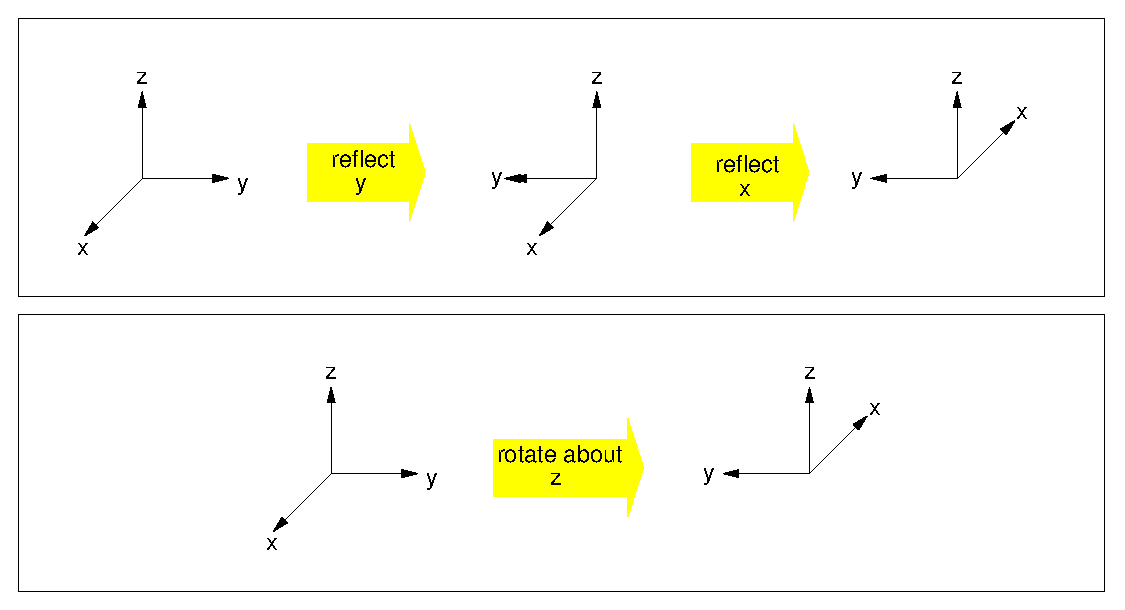
\includegraphics[height=40mm]{fig/rotate_reflect.eps}
\fi
\caption{A rotation by $\pi$ radians about the $z$-axis is equivalent
  to successive reflections about the $y$- and $x$-axes.}
\label{fig:rs_rotate_reflect}
\end{figure}

Since the transformation values for reflection symmetries are
already specified for each Cactus grid function, we can use this
information to unambiguously determine the $\pi$-rotation
transformation coefficients, without requiring that any new
information be added if the reflection symmetries have already
been defined (as is the case for any Cactus GFs which are able to
use the current \texttt{bitant}, \texttt{quadrant} and \texttt{octant}
domains).

%------------------------------------------------------------------------------
\section{\texttt{CartGrid3D} Notes}
\label{sec:rs_cartgrid3d}
%------------------------------------------------------------------------------

Two types of rotating symmetry conditions have been implemented in
\texttt{CartGrid3D} as extensions to the \texttt{grid::domain}
parameter.\\

The first, \texttt{bitant\_rotate}, defines a grid which is half-sized
along one axis, and assumes a field that is rotating about a
perpendicular axis. The half-axis is chosen using the
\texttt{bitant\_plane} parameter, which specifies the plane at which
the grid is to be cut as either ``\texttt{xy}'', ``\texttt{xz}'' or
``\texttt{yz}''. The rotation axis is chosen using the
\texttt{rotation\_axis} parameter, which takes values of
``\texttt{x}'', ``\texttt{y}'' or ``\texttt{z}''. For example, to
specify a bitant domain along the positive $y$-axis, on which fields
are rotating about the $z$-axis, the following parameters would do the
job:
\begin{verbatim}
  grid::domain = "bitant_rotate"
  grid::bitant_plane = "xz"
  grid::rotation_axis = "z"
\end{verbatim}
This setup is illustrated in Figure \ref{fig:rs_bitant_example} (a).\\

\begin{figure}
\centering
\begin{tabular}{cc}
\ifpdf
\else
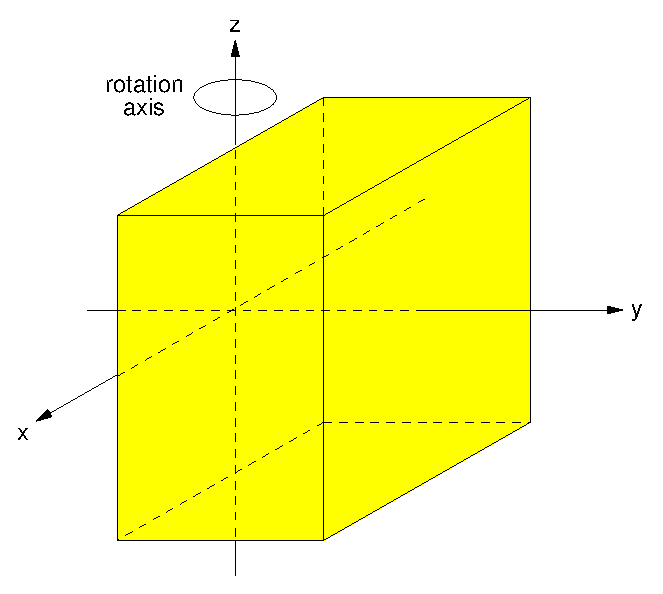
\includegraphics[height=40mm]{fig/rotate_bitant_example.eps}
\fi
&
\ifpdf
\else
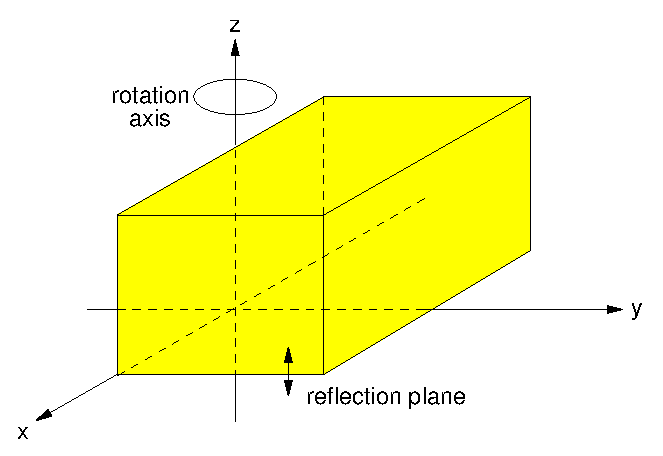
\includegraphics[height=30mm]{fig/rotate_quadrant_example.eps}
\fi
\\
(a) & (b)
\end{tabular}
\caption{Active grids for the \texttt{bitant\_rotate} and
  \texttt{quadrant\_reflect\_rotate} domains for the examples given in
  the text. (a) The given \texttt{bitant\_rotate} domain corresponds
  to the $y>0$ half-grid, with fields rotating about the $z$-axis. (b)
  The \texttt{quadrant\_reflect\_rotate} example is similar, except
  the active grid is only along the positive $z$-axis and a reflection
  symmetry is assumed in the $z=0$ plane.}
\label{fig:rs_bitant_example}
\end{figure}

The \texttt{quadrant\_reflect\_rotate} symmetry cuts two of the axes
in half so that only a quadrant of the full domain is active. A
standard reflection symmetry is applied to one of the half-planes,
while the physical fields are assumed to rotate in the other plane. To
set up such a grid which rotates about the $z$-axis and which is
reflection symmetric in the $z=0$ plane, the following parameters
would be used:
\begin{verbatim}
  grid::domain = "quadrant_reflect_rotate"
  grid::quadrant_direction = "x"
  grid::rotation_axis = "z"
\end{verbatim}
Note that the \texttt{quadrant\_direction} parameter follows the
current \texttt{CartGrid3D} standard, which defines the domain on the
\emph{positive} quadrant with the long edge aligned with the specified
axis. It is currently not possible to choose the negative quadrant.\\

Octant rotation symmetries, or the alternate quadrant symmetry (for
which the data on one half-plane is rotated onto the other), are more
difficult to implement without some generalisation of the existing
\texttt{CartGrid3D} specification of symmetry boundaries for the
reasons mentioned in the previous section.

%------------------------------------------------------------------------------
\end{document}
